\documentclass[a4,12pt]{scrartcl}

%Basic 
\usepackage[utf8]{inputenc}
\usepackage[ngerman]{babel}
\usepackage[T1]{fontenc}
%Schrift 
%\usepackage{fontspec} 
%\setmainfont{Arial} 
%Zeilenabstand
\usepackage{setspace}
\setstretch {1.3}
\usepackage{float}
\usepackage[bottom = 3.50cm]{geometry}

%Titel Seite
\usepackage{titling} %Wird benötigt damit \maketitle die Variabeln title, author und date nicht überschreibt
\title{Anforderungsspezifikation}
\subtitle{Projekt: sniffdatel}
\author{David Meister \and Giorgio Vincenti \and Samuel Krieg \and Andreas Stalder}		
 %mit /and können Personen hinzugefügt werden
\date{\today}


%Kopf, Fusszeile
\usepackage{fancyhdr}
\pagestyle{fancy}
\lhead{SW Engineering Projekt FS 2016}
\chead{}
\rhead{sniffdatel}
\lfoot{\thetitle \: v1.0 }
\cfoot{\today }
\rfoot{Seite \thepage}
\renewcommand{\headrulewidth}{0.4pt}

%Bilder
\usepackage{graphicx}

%Zeichnen
\usepackage{tikz}

%Tabellen
\usepackage{booktabs}
\usepackage{longtable}

%Codesnippets
\usepackage{listings}
\lstset{language=java,basicstyle=\footnotesize,frame=single} %backgroundcolor=\color{lightgray}

%Querformat für eine Seite
\usepackage{lscape}
\usepackage{rotating}
\usepackage{pdflscape}

%URL 
\usepackage[colorlinks=true, linkcolor=blue, urlcolor=blue, citecolor=blue]{hyperref}
\urlstyle{same} 


%Loremimpsum
\usepackage{lipsum}



\begin{document}

%\clearpage\maketitle
\begin{titlepage}
	\centering
	\vspace{5cm}
	\begin{center}
	
\includegraphics[width=0.50\textwidth]{logo.png}
	\end{center}
	{\huge\bfseries sniffdatel\par}
	\vspace{8cm}
	\raggedright
	{\bfseries SW Engineering Projekt FS 2016\par}
	{\huge\bfseries Anforderungsspezifikation\par}
	\vspace{1cm}
	{\theauthor \par}
	{\today\par}

\end{titlepage}

\section{Änderungsgeschichte}

\begin{table}[htb]
\centering
    \begin{tabular}{@{} l l l l@{}}\toprule    
    {Datum} & {Version} & {Änderung} & {Autor}\\ \midrule
    15.03.16 & 1.0 & Erstellung erster Version & Giorgio Vincenti\\ \addlinespace
    21.03.16 & 1.1 & Review ready & Alle \\
\addlinespace
    26.03.16 & 1.2 & Review ready & Alle \\
    %01.03.16 & 1.0 & Vorlage erstellt & Samuel Krieg\\ \addlinespace
    \bottomrule
    \end{tabular}
\caption{\textbf{Änderungsgeschichte}}
\end{table}
\newpage
%\thispagestyle{empty}
\tableofcontents
\newpage

\section{Einführung}
\subsection{Zweck}
Dieses Dokument beschreibt die Anforderungen mittels Use Cases und nichtfunktionalen Anforderungen.
\subsection{Gültigkeitsbereich}
Dieses Dokument ist über die gesamte Projektdauer gültig. Es wird gegebenenfalls in späteren Iterationen angepasst. Somit ist jeweils nur die neuste Version des Dokuments gültig und alte Versionen sind obsolet.
\subsection{Referenzen}
\begin{description}
  \item[Anforderungen] \hfill \\
  domainanalyse.pdf \\
\end{description}

\section{Allgemeine Beschreibung}
\subsection{Produkt Perspektive}
sniffdatel ermöglicht das Aufzeichnen und Abspielen von Voice over IP Paketen in
Echtzeit. Wireshark bietet seit langem die Möglichkeit, den Netzwerkverkehr auf
dem Interface aufzuzeichnen, RTP Streams zu filtern und diese abzuspielen. Wireshark
ist jedoch nicht in der Lage, RTP Datenpakete in Echtzeit wiederzugeben.
sniffdatel filtert RTP Streams aus dem mitgeschnittenen Netzwerkverkehr, stellt
die Streams auf einem GUI dar und spielt sie nach Wunsch ab.
\subsection{Produkt Funktion}
sniffdatel scannt Netzwerkpakete auf einem Interface. Mittels Filtertechniken werden SIP,SDP und RTP Pakete gefiltert. Aufgrund der SIP & SDP Pakete werden Sessions gefunden und aufgelistet. Zugehörige RTP Pakete werden gefiltert und deren Payload extrahiert, aufbereitet und auf einem Audio Player abgespielt.
\subsection{Benutzer Charakteristik}
Zielgruppe sind Informatikinteressierte, Studenten und Dozenten, welche sich mit der VoIP Thematik befassen möchten. Grundkenntnisse in IP-Netzwerken und VoIP sind hilfreich jedoch nicht zwingend notwendig. 
\subsection{Einschränkungen}
sniffdatel wird nur auf Linux Plattformen mit installierter libpcap (Version 0.9) unterstützt. Ausserdem wird eine JRE (Java Runtime Environment) ab Version 8 vorausgesetzt. Es werden nur RTP Pakete, welche mit G.711 im PCMA Modus codiert wurden, unterstützt.
\newpage
\section{Use Cases}
\subsection{Use Case Diagramm}
\begin{figure} [H]
	\begin{center}
	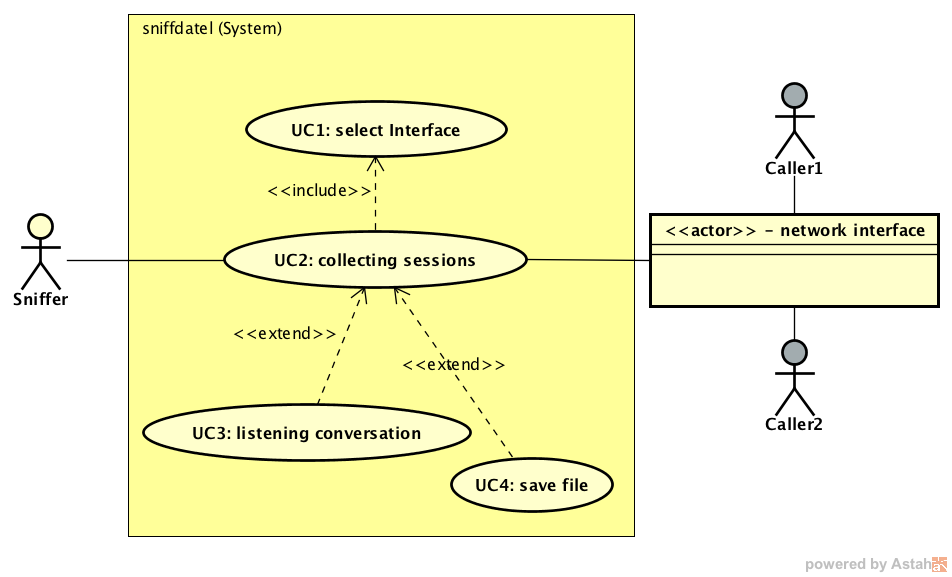
\includegraphics[width=0.80\textwidth]{./figures/UseCaseDiagramm.png}
	\caption{\textbf{Use Case Diagramm}}
	\label{Bild Referenz}
	\end{center}
\end{figure}

\subsubsection{Bemerkung}
Der Sniffer möchte gerne eine VOIP Session abhören (UC2). Damit dies möglich ist muss er zuerst ein Interface wählen auf dem er den Capture der Netzwerk Pakete durchführen möchte (UC1 - include). Falls Sessions gefunden wurden kann er diese abhören (UC3). Optional kann der Sniffer die Quelle als File abspeichern (UC4). 

\subsection{Aktoren}
\begin{table}[H]
\centering
    \begin{tabular}{@{} l l@{}}    
    {Actor} & {Beschreibung}\\ \midrule
    Sniffer & Nutzer des Systems sniffdatel\\ \addlinespace
    network interface & Liefert die benötigten Pakete\\ \addlinespace
    Callers & Telefonierende Personen\\ \bottomrule
    \end{tabular}
\caption{\textbf{Actors}}
\end{table} 

\subsection{Beschreibungen (Brief)	}
\subsubsection{UC1: select interfaces}
Der Sniffer hat die Möglichkeit Interfaces auszuwählen auf die er einen Capture starten möchte. Snifffdatel liefert dazu ein kleines GUI mit einer Auflistung der vorhandenen Netzwerk Interfaces. Der Sniffer wählt dazu eines aus und bestätigt die Auswahl. Der Sniffer kann das GUI auch jederzeit wieder verlassen mit cancel. 
\subsubsection{UC2: collecting sessions}
Der Sniffer kann einen Capture Vorgang starten um eingehende Datenpakete zu analysieren. Sniffdatel listet dabei vorhandene VOIP Sessions im Netzwerk auf in einer Liste. Der Sniffer hat die Möglichkeit eine Session auszuwählen. Der Sniffer hat ebenso die Möglichkeit einen Capture Restart durchzuführen (starten Vorgang neu), oder den Caputure Vorgang abzubrechen. 
\subsubsection{UC3: listening conversations}
Der Sniffer hat die Möglichkeit die von Sniffdatel aufgelistete Sessions abzuspielen mittels Play (trigger). Sniffdatel startet jetzt eine Audio Wiedergabe der ausgewählten Session. Der Sniffer hat die Möglichkeit die Wiedergabe zu stoppen, oder eine andere Session abzuhören. Sniffdatel beendet die Wiedergabe automatisch sobald keine weiteren eingehende Pakete zu einer Session gefunden wurden. 
\subsubsection{UC4: save file}
Der Sniffer hat die Möglichkeit eine laufende Session als Datei lokal abzuspeichern. Für diesen Vorgang muss der Snffer nicht die Quelle abhören, sondern kann statt Play den Button Save drücken. Es handelt sich hierbei um ein optionales Feature, welches nur bei ausreichender Zeit berücksichtigt wird. 
\newpage
\subsection{Beschreibungen (Fully Dressed)	}
\subsubsection{UC1: select interfaces}
\begin{description}
  \item[Primary Actor:] Sniffer
  \item[Postcondition:] Interface ausgewählt und bestätigt
  \item[Stakeholder and Interests:] \hfill
  	\begin{itemize}
  		\item Sniffer: will Gespräch von Teilnehmer abhören 
  	\end{itemize}
  \item[Goal:] Gewünschtes Interfaces für Sniffing ausgewählt
  \item[Trigger:] Clickevent auf "capture interface"
  \item[Main Success Scenario (or Basic Flow):] \hfill
  	\begin{enumerate}
  		\item Snifferdatel liefert Interfaceauswahl
  		\item Sniffer wählt gewünschte Interfaces aus
  		\item Sniffdatel markiert gewünschtes Interfaces
  		\item Sniffer bestätigt Auswahl
  		\item Sniffdatel aktiviert markierte Interfaces (falls welche ausgewählt)
	\end{enumerate}
  \item[Extensions (or Alternative Flows):] \hfill
  	\begin{itemize}
		\item[*a.] jederzeit - Applikation stürzt ab
  			\begin{enumerate}
  				\item Sniffer startet Applikation neu 		 
			\end{enumerate}
		\item[1a.] Sniffdatel liefert keine Interfaces
  			\begin{enumerate}
  				\item Sniffer startet Applikation neu 		 
			\end{enumerate}
		\item[1-3a.] Sniffer bricht Vorgang ab
  			\begin{enumerate}
  				\item Sniffdatel schliesst Interfaceauswahl		 
			\end{enumerate}	
	\end{itemize}
\end{description}

\subsubsection{UC2: collecting sessions}
	\begin{description}
		\item[Primary Actor:] Sniffer
		\item[Precondition:] Sniffdatel gestartet
  		\item[Stakeholder and Interests:] \hfill
  			\begin{itemize}
  				\item Sniffer: will VOIP-Sessions sammeln
  				\item VOIP Teilnehmer: sind unwissend über Vorgänge des Tools
  			\end{itemize}
 		\item[Goal:] Analyse von VOIP Sessions
  		\item[Trigger:] Sniffer möchte das Programm verwenden
 		\item[Main Success Scenario (or Basic Flow):] \hfill
  			\begin{enumerate}
  				\item Sniffdatel zeigt GUI an
				\item Sniffer Clickt \grqq capture interface\grqq
					\begin{description}
  						\item[] Siehe Sub-UC \grqq select interface\grqq 
  					\end{description}
				\item Sniffer Klickt \grqq start capture\grqq 
				\item Sniffdatel Listet Sessions auf
				\item Sniffer wählt Session aus
				\item Sniffdatel markiert gwünschte Session
				\item Sniffer klickt \grqq start audio\grqq 
					\begin{description}
  						\item[] Siehe Sub-UC \grqq listening conversation\grqq 
  					\end{description}				
				\item Sniffer beendet Sniffdatel
			\end{enumerate}
  		\item[Extensions (or Alternative Flows):] \hfill  
  			\begin{itemize}
				\item[*a.] jederzeit - VOIP Verbindungsaufbau findet statt
  					\begin{enumerate}
  						\item Sniffdatel nimmt neue Verbindung in Liste auf
					\end{enumerate}
				\item[*b.] jederzeit - VOIP Verbindung wird beendet
  					\begin{enumerate}
  						\item Sniffdatel kennzeichnet beendete Verbindung 
					\end{enumerate}
				\item[*c.]  jederzeit - Sniffdatel absturz
  					\begin{enumerate}
  						\item Sniffer muss Software neustarten
					\end{enumerate}
				\item[4-8a.] Sniffer klickt \grqq restart caputre\grqq 
  					\begin{enumerate}
  						\item Sniffdatel startet Capture neu
					\end{enumerate}
				\item[4-8b.] Sniffer klickt \grqq stop capture\grqq 
  					\begin{enumerate}
  						\item Sniffdatel beendet Capture
					\end{enumerate}
					
			\end{itemize}
\end{description}

\subsubsection{UC3: listening conversations}
	\begin{description}
		\item[Primary Actor:] Sniffer
		\item[Postcondition:] Wiedergabe ist beendet
  		\item[Stakeholder and Interests:] \hfill
  			\begin{itemize}
  				\item Sniffer: will Gespräch von Teilnehmer abhören
  			\end{itemize}
 		\item[Goal:] Gespräch erfolgreich abgehört
  		\item[Trigger:] Clickevent auf \grqq start audio\grqq 
 		\item[Main Success Scenario (or Basic Flow):] \hfill
  			\begin{enumerate}
  				\item Sniffdatel startet Wiedergabe der ausgewählte Session
				\item Sniffer beendet Wiedergabe
			\end{enumerate}
  		\item[Extensions (or Alternative Flows):] \hfill  
  			\begin{itemize}
				\item[*a.] jederzeit - Applikation stürtzt ab
  					\begin{enumerate}
  						\item Sniffer startet Applikation neu
					\end{enumerate}
				\item[*b.] jederzeit - Sniffer klickt \grqq stop capture\grqq 
  					\begin{enumerate}
  						\item Sniffdatel beendet Wiedergabe
					\end{enumerate}
				\item[1a.] Sniffdatel startet Wiedergabe nicht
  					\begin{enumerate}
  						\item Sniffer versucht Wiedergabe erneut zu starten
					\end{enumerate}
				\item[1b.] Sniffer wählt andere Session
  					\begin{enumerate}
  						\item Sniffdatel startet Wiedergabe der ausgewählte Session
					\end{enumerate}
				\item[2a.] Sniffdatel beendet Wiedergabe					
			\end{itemize}
\end{description}
\subsubsection{UC4: save file}
Da es sich bei UC4 um ein optionales Feature handelt, wurde auf eine Fully Dressed Beschreibung verzichtet. Siehe Kapitel 4.3.4 UC4: save file für eine Kurzbeschreibung. 
\section{Nichtfunktionale Anforderungen}
In diesem Kapitel behandeln wir die nichtfunktionalen Anforderungen an das Projekt. Wir behandeln Aspekte und Anforderungen aus den Bereichen Performance, Qualität, Schnittstellen und Randbedingungen.
\subsection{Performance}
\subsubsection{Ladezeiten}
Die Zeit zum Aufstarten des Programms darf 10 Sekunden nicht überschreiten. Beim Abspielen des aufgezeichneten VoIP Verkehrs darf die Verzögerung nicht länger als 1 Sekunde betragen (Real-Time).
\subsubsection{Datenübertragungsraten}
Sniffdatel ist ein lokal installiertes Tool zum Aufzeichnen und Abspielen von VoIP Verkehr. Das Tool soll bei Datenübertragungsraten von und bis 100Mbit/s stabil funktionieren.
\subsection{Qualität}
Bei der Softwarequalität stützen wir uns auf die ISO/IEC 9126 Norm. Es werden die Merkmale Funktionalität, Zuverlässigkeit, Benutzbarkeit, Effizienz, Wartbarkeit und Übertragbarkeit aufgeführt.
\subsubsection{Funktionalität}
Durch die Java Technologie wird sichergestellt, dass Sniffdatel auf allen gängigen Betriebssystemen funktioniert. Vorgesehen sind vorerst jedoch nur Clientgeräte (PC/Notebook) mit gängigen und aktuellen UNIX Betriebssystemen. 
\subsubsection{Zuverlässigkeit}
Da es sich bei sniffdatel um ein lokales Programm handelt, welches in keinster Weise businesskritisch ist, sind keine erhöhten Anforderungen an die Zuverlässigkeit des Systems gegeben. Eine Stabilität unter den gegebenen Rahmenbedingungen ist trotzdem Pflicht. Besonderes Augenmerk ist dem Buffer-Mechanismus zu schenken. Bei fehlenden RTP Paketen, oder bei zu hoher Netzwerklast darf das Programm nicht abstürzen. Out-of-Order RTP Pakete oder Verzögerungen sollen durch einen guten Buffer-Mechanismus korrigiert werden.
\subsubsection{Benutzbarkeit}
Ein einfaches und intuitives Bedienen des Programms ist sehr wichtig für uns. Wir verzichten auf aufwändige GUI Elemente und beschränken uns auf wesentliche Funktionen und Anzeigen. Unser Ziel ist, dass weniger versierte Benutzer das Programm ohne Einarbeitungszeit bedienen können. 
\subsubsection{Effizienz}
Siehe Kapitel Performance.
\subsubsection{Wartbarkeit}
Momentan sind keine Erweiterungen für sniffdatel geplant. Zusätzliche Features sind jedoch gut denkbar. Man könnte z.B. eine Entschlüsselungsfunktion für verschlüsselten RTP Payload einbauen oder zusätzliche Funktionen für die Audiowiedergabe (stop, zurück, etc.) einbauen. Unser Ziel ist es, solche Zusatzfunktionen für spätere Anpassungen möglich zu machen.
\subsubsection{Übertragbarkeit}
Dank der Java Technologie sind die Programme grundsätzlich Plattformunabhängig. Wir unterstützen vorerst jedoch nur UNIX Betriebssysteme, damit wir Probleme diesbezüglich vermeiden möchten.
\subsection{Datenschutz}
Sniffdatel speichert keine personenbezogenen Daten. Die abgehörten Gespräche werden nicht dauerhaft gespeichert. Es kann jedoch nicht verhindert werden, dass der Benutzer des Systems die Software missbräuchlich verwendet (z.B. Abhören von Gesprächen Dritter) oder die abgespielten Gespräche mit einem anderen Werkzeug abspeichert.
\subsection{Schnittstellen}
\subsubsection{Benutzerschnittstellen}
Die Steuerung des Programms ist nur mit der Maus vorgesehen.
\subsubsection{Netzwerkschnittstellen}
Im Programm können alle vom Betriebssystem erkannten Netzwerkinterfaces verwendet werden.
\end{document}

